\documentclass[twoside]{book}

% Packages required by doxygen
\usepackage{fixltx2e}
\usepackage{calc}
\usepackage{doxygen}
\usepackage[export]{adjustbox} % also loads graphicx
\usepackage{graphicx}
\usepackage[utf8]{inputenc}
\usepackage{makeidx}
\usepackage{multicol}
\usepackage{multirow}
\PassOptionsToPackage{warn}{textcomp}
\usepackage{textcomp}
\usepackage[nointegrals]{wasysym}
\usepackage[table]{xcolor}

% Font selection
\usepackage[T1]{fontenc}
\usepackage[scaled=.90]{helvet}
\usepackage{courier}
\usepackage{amssymb}
\usepackage{sectsty}
\renewcommand{\familydefault}{\sfdefault}
\allsectionsfont{%
  \fontseries{bc}\selectfont%
  \color{darkgray}%
}
\renewcommand{\DoxyLabelFont}{%
  \fontseries{bc}\selectfont%
  \color{darkgray}%
}
\newcommand{\+}{\discretionary{\mbox{\scriptsize$\hookleftarrow$}}{}{}}

% Page & text layout
\usepackage{geometry}
\geometry{%
  a4paper,%
  top=2.5cm,%
  bottom=2.5cm,%
  left=2.5cm,%
  right=2.5cm%
}
\tolerance=750
\hfuzz=15pt
\hbadness=750
\setlength{\emergencystretch}{15pt}
\setlength{\parindent}{0cm}
\setlength{\parskip}{3ex plus 2ex minus 2ex}
\makeatletter
\renewcommand{\paragraph}{%
  \@startsection{paragraph}{4}{0ex}{-1.0ex}{1.0ex}{%
    \normalfont\normalsize\bfseries\SS@parafont%
  }%
}
\renewcommand{\subparagraph}{%
  \@startsection{subparagraph}{5}{0ex}{-1.0ex}{1.0ex}{%
    \normalfont\normalsize\bfseries\SS@subparafont%
  }%
}
\makeatother

% Headers & footers
\usepackage{fancyhdr}
\pagestyle{fancyplain}
\fancyhead[LE]{\fancyplain{}{\bfseries\thepage}}
\fancyhead[CE]{\fancyplain{}{}}
\fancyhead[RE]{\fancyplain{}{\bfseries\leftmark}}
\fancyhead[LO]{\fancyplain{}{\bfseries\rightmark}}
\fancyhead[CO]{\fancyplain{}{}}
\fancyhead[RO]{\fancyplain{}{\bfseries\thepage}}
\fancyfoot[LE]{\fancyplain{}{}}
\fancyfoot[CE]{\fancyplain{}{}}
\fancyfoot[RE]{\fancyplain{}{\bfseries\scriptsize Generated by Doxygen }}
\fancyfoot[LO]{\fancyplain{}{\bfseries\scriptsize Generated by Doxygen }}
\fancyfoot[CO]{\fancyplain{}{}}
\fancyfoot[RO]{\fancyplain{}{}}
\renewcommand{\footrulewidth}{0.4pt}
\renewcommand{\chaptermark}[1]{%
  \markboth{#1}{}%
}
\renewcommand{\sectionmark}[1]{%
  \markright{\thesection\ #1}%
}

% Indices & bibliography
\usepackage{natbib}
\usepackage[titles]{tocloft}
\setcounter{tocdepth}{3}
\setcounter{secnumdepth}{5}
\makeindex

% Hyperlinks (required, but should be loaded last)
\usepackage{ifpdf}
\ifpdf
  \usepackage[pdftex,pagebackref=true]{hyperref}
\else
  \usepackage[ps2pdf,pagebackref=true]{hyperref}
\fi
\hypersetup{%
  colorlinks=true,%
  linkcolor=blue,%
  citecolor=blue,%
  unicode%
}

% Custom commands
\newcommand{\clearemptydoublepage}{%
  \newpage{\pagestyle{empty}\cleardoublepage}%
}

\usepackage{caption}
\captionsetup{labelsep=space,justification=centering,font={bf},singlelinecheck=off,skip=4pt,position=top}

%===== C O N T E N T S =====

\begin{document}

% Titlepage & ToC
\hypersetup{pageanchor=false,
             bookmarksnumbered=true,
             pdfencoding=unicode
            }
\pagenumbering{roman}
\begin{titlepage}
\vspace*{7cm}
\begin{center}%
{\Large My Project }\\
\vspace*{1cm}
{\large Generated by Doxygen 1.8.11}\\
\end{center}
\end{titlepage}
\clearemptydoublepage
\tableofcontents
\clearemptydoublepage
\pagenumbering{arabic}
\hypersetup{pageanchor=true}

%--- Begin generated contents ---
\chapter{Hierarchical Index}
\section{Class Hierarchy}
This inheritance list is sorted roughly, but not completely, alphabetically\+:\begin{DoxyCompactList}
\item \contentsline{section}{Grayscale\+Client}{\pageref{classGrayscaleClient}}{}
\item Remote\begin{DoxyCompactList}
\item \contentsline{section}{Grayscale\+Interface}{\pageref{interfaceGrayscaleInterface}}{}
\begin{DoxyCompactList}
\item \contentsline{section}{Grayscale\+Server}{\pageref{classGrayscaleServer}}{}
\end{DoxyCompactList}
\end{DoxyCompactList}
\item Unicast\+Remote\+Object\begin{DoxyCompactList}
\item \contentsline{section}{Grayscale\+Server}{\pageref{classGrayscaleServer}}{}
\end{DoxyCompactList}
\end{DoxyCompactList}

\chapter{Class Index}
\section{Class List}
Here are the classes, structs, unions and interfaces with brief descriptions\+:\begin{DoxyCompactList}
\item\contentsline{section}{\hyperlink{classGrayscaleClient}{Grayscale\+Client} }{\pageref{classGrayscaleClient}}{}
\item\contentsline{section}{\hyperlink{interfaceGrayscaleInterface}{Grayscale\+Interface} }{\pageref{interfaceGrayscaleInterface}}{}
\item\contentsline{section}{\hyperlink{classGrayscaleServer}{Grayscale\+Server} }{\pageref{classGrayscaleServer}}{}
\end{DoxyCompactList}

\chapter{Class Documentation}
\hypertarget{classGrayscaleClient}{}\section{Grayscale\+Client Class Reference}
\label{classGrayscaleClient}\index{Grayscale\+Client@{Grayscale\+Client}}
\subsection*{Static Public Member Functions}
\begin{DoxyCompactItemize}
\item 
static void \hyperlink{classGrayscaleClient_a560bbf8aa076b373ce660ef446750170}{main} (String\mbox{[}$\,$\mbox{]} args)  throws I\+O\+Exception 
\item 
static Linked\+List$<$ int\mbox{[}$\,$\mbox{]}$>$ \hyperlink{classGrayscaleClient_a6d22c0e1ee10ec06dabbd248bf8b10eb}{split\+Image} (Buffered\+Image image, int split\+Size)  throws I\+O\+Exception 
\item 
static Buffered\+Image {\bfseries join\+Images} (Linked\+List$<$ int\mbox{[}$\,$\mbox{]}$>$ split\+Images\+Bytes, int width, int height, int type, int split\+Size)\hypertarget{classGrayscaleClient_ade172cb7aff4bb2b38d1eefa5a54d3e1}{}\label{classGrayscaleClient_ade172cb7aff4bb2b38d1eefa5a54d3e1}

\item 
static Thread {\bfseries convert\+Image} (\hyperlink{interfaceGrayscaleInterface}{Grayscale\+Interface} grayscale, Linked\+List$<$ int\mbox{[}$\,$\mbox{]}$>$ split\+Images\+Bytes, int index)\hypertarget{classGrayscaleClient_a4884430c9fa4d2d2bbaa35e6887ddb7d}{}\label{classGrayscaleClient_a4884430c9fa4d2d2bbaa35e6887ddb7d}

\end{DoxyCompactItemize}


\subsection{Member Function Documentation}
\index{Grayscale\+Client@{Grayscale\+Client}!main@{main}}
\index{main@{main}!Grayscale\+Client@{Grayscale\+Client}}
\subsubsection[{\texorpdfstring{main(\+String[] args)}{main(String[] args)}}]{\setlength{\rightskip}{0pt plus 5cm}static void Grayscale\+Client.\+main (
\begin{DoxyParamCaption}
\item[{String\mbox{[}$\,$\mbox{]}}]{args}
\end{DoxyParamCaption}
) throws I\+O\+Exception\hspace{0.3cm}{\ttfamily [inline]}, {\ttfamily [static]}}\hypertarget{classGrayscaleClient_a560bbf8aa076b373ce660ef446750170}{}\label{classGrayscaleClient_a560bbf8aa076b373ce660ef446750170}
Lendo os n servidores.

Lendo imagem através do diretório recebido.

Pegando tipo, width e height da imagem.

Separando a imagem em n partes iguais, de acordo com o número de servidores a serem utilizados.

Inicializando as interfaces.

Convertendo partes da imagem em diferentes threads.

Esperando que todas as thread terminem de executar antes de continuar com a main.

Juntando todas as partes da imagem convertida.

Calculando o tempo gasto para a conversão.\index{Grayscale\+Client@{Grayscale\+Client}!split\+Image@{split\+Image}}
\index{split\+Image@{split\+Image}!Grayscale\+Client@{Grayscale\+Client}}
\subsubsection[{\texorpdfstring{split\+Image(\+Buffered\+Image image, int split\+Size)}{splitImage(BufferedImage image, int splitSize)}}]{\setlength{\rightskip}{0pt plus 5cm}static Linked\+List$<$int\mbox{[}$\,$\mbox{]}$>$ Grayscale\+Client.\+split\+Image (
\begin{DoxyParamCaption}
\item[{Buffered\+Image}]{image, }
\item[{int}]{split\+Size}
\end{DoxyParamCaption}
) throws I\+O\+Exception\hspace{0.3cm}{\ttfamily [inline]}, {\ttfamily [static]}}\hypertarget{classGrayscaleClient_a6d22c0e1ee10ec06dabbd248bf8b10eb}{}\label{classGrayscaleClient_a6d22c0e1ee10ec06dabbd248bf8b10eb}
pegando width e height da imagem

The documentation for this class was generated from the following file\+:\begin{DoxyCompactItemize}
\item 
Grayscale\+Client.\+java\end{DoxyCompactItemize}

\hypertarget{interfaceGrayscaleInterface}{}\section{Grayscale\+Interface Interface Reference}
\label{interfaceGrayscaleInterface}\index{Grayscale\+Interface@{Grayscale\+Interface}}


Inheritance diagram for Grayscale\+Interface\+:
\nopagebreak
\begin{figure}[H]
\begin{center}
\leavevmode
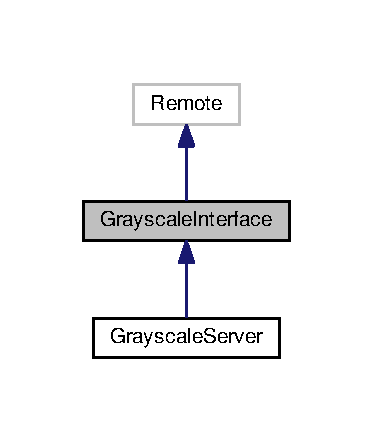
\includegraphics[width=179pt]{interfaceGrayscaleInterface__inherit__graph}
\end{center}
\end{figure}


Collaboration diagram for Grayscale\+Interface\+:
\nopagebreak
\begin{figure}[H]
\begin{center}
\leavevmode
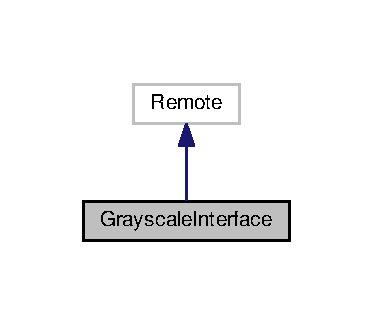
\includegraphics[width=179pt]{interfaceGrayscaleInterface__coll__graph}
\end{center}
\end{figure}
\subsection*{Public Member Functions}
\begin{DoxyCompactItemize}
\item 
int\mbox{[}$\,$\mbox{]} {\bfseries convert} (int\mbox{[}$\,$\mbox{]} image)  throws Remote\+Exception	\hypertarget{interfaceGrayscaleInterface_aff44e0d3dc8bba6abfff41782864b373}{}\label{interfaceGrayscaleInterface_aff44e0d3dc8bba6abfff41782864b373}

\end{DoxyCompactItemize}


The documentation for this interface was generated from the following file\+:\begin{DoxyCompactItemize}
\item 
Grayscale\+Interface.\+java\end{DoxyCompactItemize}

\hypertarget{classGrayscaleServer}{}\section{Grayscale\+Server Class Reference}
\label{classGrayscaleServer}\index{Grayscale\+Server@{Grayscale\+Server}}


Inheritance diagram for Grayscale\+Server\+:
\nopagebreak
\begin{figure}[H]
\begin{center}
\leavevmode
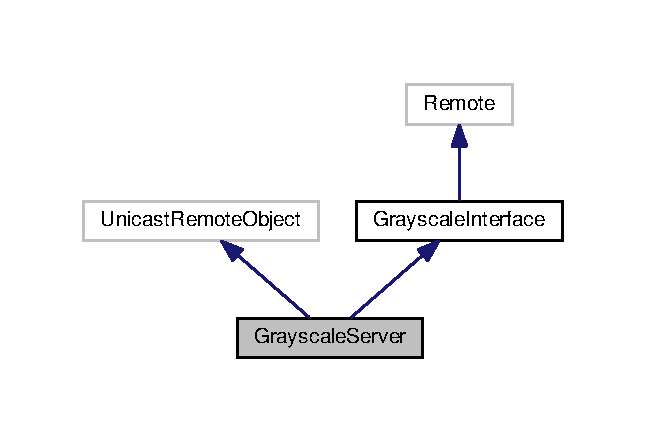
\includegraphics[width=310pt]{classGrayscaleServer__inherit__graph}
\end{center}
\end{figure}


Collaboration diagram for Grayscale\+Server\+:
\nopagebreak
\begin{figure}[H]
\begin{center}
\leavevmode
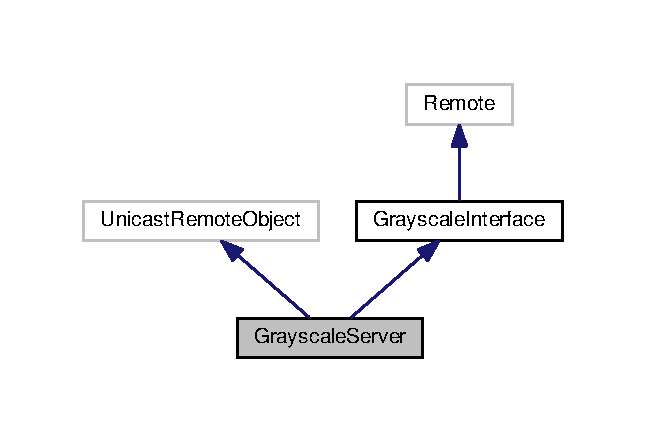
\includegraphics[width=310pt]{classGrayscaleServer__coll__graph}
\end{center}
\end{figure}
\subsection*{Public Member Functions}
\begin{DoxyCompactItemize}
\item 
int\mbox{[}$\,$\mbox{]} {\bfseries convert} (int\mbox{[}$\,$\mbox{]} image)  throws Remote\+Exception \hypertarget{classGrayscaleServer_a7eb7845b86bad3a7a1c66f6979a3c00b}{}\label{classGrayscaleServer_a7eb7845b86bad3a7a1c66f6979a3c00b}

\end{DoxyCompactItemize}
\subsection*{Static Public Member Functions}
\begin{DoxyCompactItemize}
\item 
static void {\bfseries main} (String\mbox{[}$\,$\mbox{]} args)\hypertarget{classGrayscaleServer_ab292e713596db3cea2c2abb570441edf}{}\label{classGrayscaleServer_ab292e713596db3cea2c2abb570441edf}

\end{DoxyCompactItemize}


The documentation for this class was generated from the following file\+:\begin{DoxyCompactItemize}
\item 
Grayscale\+Server.\+java\end{DoxyCompactItemize}

%--- End generated contents ---

% Index
\backmatter
\newpage
\phantomsection
\clearemptydoublepage
\addcontentsline{toc}{chapter}{Index}
\printindex

\end{document}
